% Template for ICIP-2015 paper; to be used with:
%          spconf.sty  - ICASSP/ICIP LaTeX style file, and
%          IEEEbib.bst - IEEE bibliography style file.
% --------------------------------------------------------------------------
\documentclass{report}
\usepackage{amsmath,graphicx}
\usepackage{color}
\usepackage{pict2e}
\usepackage{dsfont}
\usepackage{stmaryrd}
\usepackage{caption}
\usepackage{subcaption}
\usepackage{geometry}
\usepackage{multirow}
\usepackage{url}
\usepackage{tikz}
\usetikzlibrary{decorations.pathreplacing}
% \usepackage{pdfpages}

\usepackage[linktoc=all]{hyperref}
\hypersetup{
    colorlinks,
    citecolor=black,
    filecolor=black,
    linkcolor=black,
    urlcolor=black
}

\geometry{
a4paper,
total={210mm,297mm},
left=25mm,
right=25mm,
top=25mm,
bottom=25mm,
}


% Example definitions.
% --------------------
\def\x{{\mathbf x}}
\def\L{{\cal L}}

% Title.
% ------
\title{Convolutional Neural Networks - a brief introduction}
\author{Michael BLOT, Thibaut DURAND, Marion CHEVALIER}
\date{June 2015}

\pagestyle{headings}

%
%\name{M. Chevalier$^{(1,2)}$, N. Thome$^{(1)}$, M. Cord$^{(1)}$, J. Fournier$^{(2)}$, G. Henaff$^{(2)}$, E. Dusch$^{(2)}$}
%\address{(1) Sorbonne universites, UPMC Univ Paris 06, UMR 7606, LIP6, F-75005, Paris, France\\
%	 (2) Thales Optronique S.A.S., 2 avenue Gay-Lussac, 78990 Elancourt, France}
%
%
%\setlength{\belowcaptionskip}{-50cm}
\begin{document}
%\ninept
%
\maketitle

\tableofcontents




%===========================================================
\chapter{Introduction}

\section{What is a CNN?}
\label{intro}

\begin{itemize}
 \item General biblio
 \item Can be used as feature extractor or complete system (feature + classif)
 \item In CNN, filters (weights) learned / in traditional Computer Vision, weights handcrafted (predetermined)
 \item CNN general scheme
 \item Each ``step'' can be seen as an ``independent'' block + scheme 
 \item Convolutions $\sim$ representation / fully connected $\sim$ classification
 \item Last layers = N classes
\end{itemize}

In the following, each block is described with $\mathbf{x}$ the block input vector 


\section{Network training}
\begin{itemize}
 \item Backprop principle
 \item General derivation equation (reference to the general scheme notations in \ref{intro})
 \item General update equation
 \item Short explanation about all learning parameters (learning rate, momentum, weight decay...)
 \item Each block can be derived ``independently'' / each block is an ``independent'' part of the backprop chain
 \item[$\rightarrow$] In the following, we describe, for each computational block, its forward formulation $y = f(x)$ and its backward formulation
 \item dropout
\end{itemize}



%===========================================================
\chapter{Architecture blocks}
\label{blocks}

We now describe the different standard computational blocks encountered in CNNs. 
We represent each block as a function $f$ which input is a matrix $\mathbf{x}$, and which output is a matrix
$\mathbf{y}$. The weights of the filter, when they exist, are denoted as the matrix $\mathbf{w}$.

  \begin{center}
  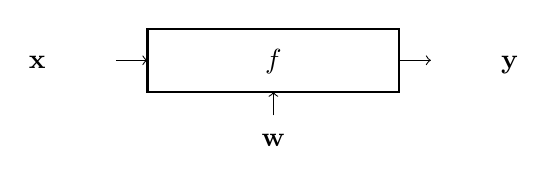
\begin{tikzpicture}
    \pgftext[base, x=   0cm, y= 0cm] {$f$}; 
    \pgftext[base, x=  -3cm, y= 0cm] {$\mathbf{x}$}; 
    \pgftext[base, x=   3cm, y= 0cm] {$\mathbf{y}$}; 
    \pgftext[base, x=   0cm, y=-1cm] {$\mathbf{w}$}; 
    \draw[black,thick] (-1.6cm,-0.3cm) rectangle (1.6cm,0.5cm); 
    \draw[->] ( -2cm, 0.1cm) -- (-1.6cm, 0.1cm);
    \draw[->] (1.6cm, 0.1cm) -- (   2cm, 0.1cm);
    \draw[->] (  0cm,-0.6cm) -- (   0cm,-0.3cm);
  \end{tikzpicture}
  \end{center}
  
For each block, we describe its formulation in a forward computation $\mathbf{y} = f(\mathbf{x},\mathbf{w})$.
We also provide the derivative of its output with respect to its input $\frac{dy}{dx}$. In order to be more explicit, we mention here the derivative 
of each output component with respect to each input component: $\frac{dy_{k_2}}{dx_{k_1}}$, where $k_1$ describes the dimension of the block input 
$\mathbf{x}$ and $k_2$ describes the dimension of the block output $\mathbf{y}$.  
These formulations can then be replaced in the equation %\ref{}
, allowing to compute the derivative of the CNN output $z$ with respect to each 


In the following section, $\delta$ is the Kronecker symbol: 
\begin{align}
  \delta_{proposition} &= 1 \hspace{0.2cm} \text{if} \hspace{0.2cm}  proposition \hspace{0.2cm} \text{is true}, \nonumber \\ 
                       &= 0 \hspace{0.2cm} \text{otherwise}. \nonumber
\end{align}

\section{Convolutions}
\begin{itemize}
 \item Forward / backward formulation
 \item Padding
\end{itemize}

\paragraph{Summary. }
\begin{itemize}
	\item Volume of size $W_i*H_i*D_i$ as input
	\item Requires four hyper-parameters :
    \begin{itemize}
    	\item number of filters (or kernels) K,
        \item spatial extent F,
        \item stride S,
        \item zero padding P
    \end{itemize}
	\item Produce a volume of size $W_o*H_o*D_o$ where :
    \begin{itemize}
		\item $W_o = \frac{W_i - F + 2*P}{S} + 1$
		\item $H_o = \frac{H_i - F + 2*P}{S} + 1$
		\item $D_o = K$
    \end{itemize}
    \item Number of weights equal to $F*F*D_i$ per filter
    \item Number of biases equal to 1 per filter
\end{itemize}


\paragraph{Padding. }

\begin{figure}
 \begin{center}
  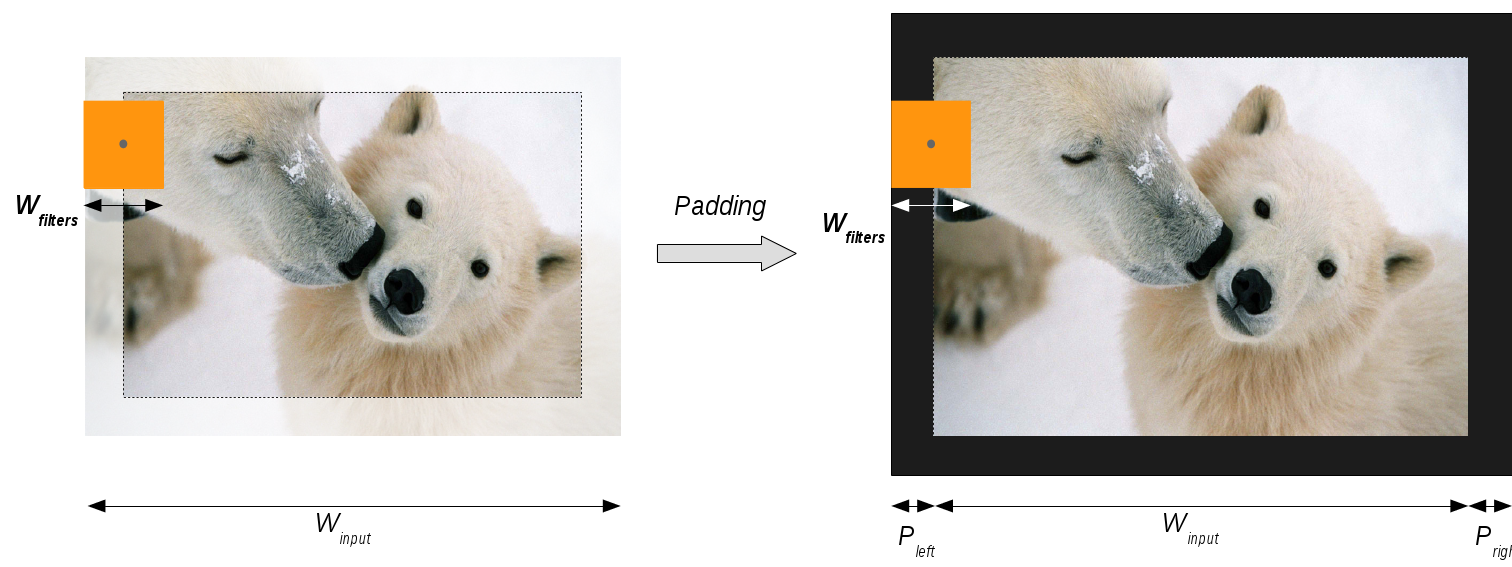
\includegraphics[width=16cm]{images/padding.png}
 \end{center}
  \caption{
  \label{fig:padding}
  Padding. Due to the filters width, the filters cannot be applied to the borders of the image. Padding consists in enlarging the 
  image by zeros, which enables the filters to be applied to the \textit{entire} image (including borders). 
  }
\end{figure}

In figure \ref{fig:padding}, we represent the padding (or ``zero-padding'') process. It consists in artificially augmenting the size of the input image (or map) in order to avoid border effects. Indeed, due to the width of the convolutional filters applied to the input maps, the center of the filters (represented as the grey dot in figure \ref{fig:padding}) cannot be at the border of the image. 
Convolutional padding is usually used to avoid a spatial reduction (downsampling) which is left for the pooling layers only. For instance, we have an image of size $30*30*3$ that we convolve using 128 filters of size $3*3*3$  with padding 0 and stride 1. The size of the output map will be $28*28*128$. If we had used a padding 1, it would have been $30*30*128$.

The total number of possible positions for the center of the filters is: 
\begin{align}
 W_{input} - W_{filters} + 1 \nonumber
\end{align}

However, if zeros are added at the border of the image, the center of the filters can be positionned at the border of the input image, so that the filters do not suffer from border effects. 
The total number of positions for the center of the filters is then: 
\begin{align}
 \underbrace{W_{input} + P_{left} + P_{right}}_{\textit{zero-padded image}} - W_{filters} + 1 \nonumber
\end{align}

Obviously, this process is applied in the same fashion no matter if the input is a set of maps or an 
image.




\paragraph{Volume of an output map. }

\begin{figure}
 \begin{center}
  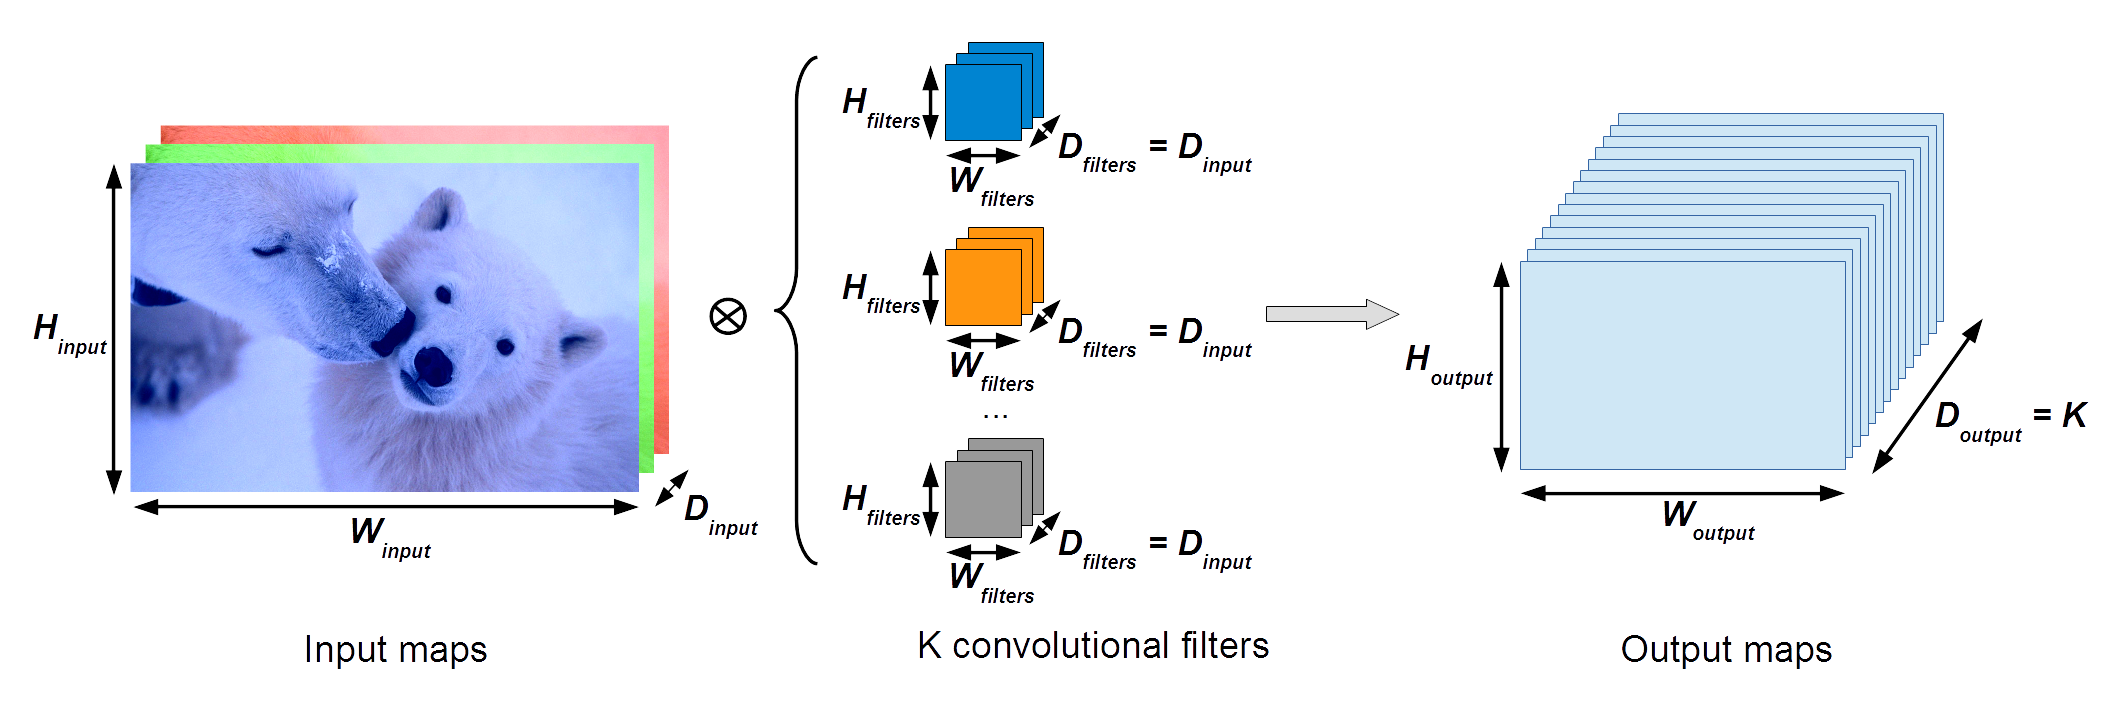
\includegraphics[width=16cm]{images/schema_conv.png}
 \end{center}
  \caption{
  \label{fig:conv}Convolution scheme. 
  }
\end{figure}

An output map is characterized by three parameters : depth, width and height. It is the result of a convolution apply to an input map made of the same parameters. For instance, an RGB image of size $227*227$ can be considered as an input map of size $[227*227*3]$.
In figure \ref{fig:conv}, we represent the general scheme for convolution. 
The width and height of the ouput map is used in particular when you want to compute the number of neurons which compose the fully connected layers. It is calculated as follow : 
\begin{align}
 W_{output} = \lfloor \frac{W_{input} + P_{left} + P_{right} - W_{filters}}{\delta_{filters}} \rfloor + 1 \nonumber
\end{align}
An equation can also be written for the height of the output map. However in the most popular cases width and height are equal.

For instance, the Alex net architecture that won the ImageNet challenge in 2012 take as input images of size $[227x227x3]$. The first convolutional layer uses neurons with receptive field size $W_{filters} = 11$, stride $\delta_{filters} = 4$ and padding $P_{left} = P_{right} = 0$. So the convolutional layer has an output volume of size $[55*55*96]$ ($\frac{227 + 0 + 0 - 11}{4} + 1 = 55$) and each of the $55*55*96$ neurons are connected to a region of size $[11*11*3]$.

The depth of the output map is however equivalent to the number of filters. Indeed, one map is produced for each of the $K$ filter banks; these response maps are then stocked as a 3D matrix.


\paragraph{Number of parameters. }

Using the real-world example from above, we can consider the first layer of AlexNet. The later is composed of 96 filters (or kernels) of size $[11*11*3]$, for a total of $96*11*11*3 = 34,848$ unique weights and 96 biases. In fact, each filter is applied to every group of $11*11*3$ pixels (considering stride and padding) to compute the final $55*55$ output map per filter, for a total of $55*55*96$ output. It is possible to find in the literature the concept of \textit{Parameter Sharing Scheme} to illustrate this fact.


\paragraph{Implementation. }

Also different implementations  of convolution can be found in the most famous libraries. For instance, the SpatialConvolutionMM from Torch nn constructs the Toeplitz matrix and does matrix multiplication. As the number of parameters does not change, one can try different implementations in order to improve efficiency.

\paragraph{Fully Connected layers. }

LeCun has once said that the concept of FC layers shouldn't be used when speaking about ConvNet, because FC layers can be seen as CONV layers with filters of size $[1*1]$.

\paragraph{Note. }

One can find some layers called TemporalConvolution, SpatialConvolution, or VolumetricConvolution. They are respectively used for processing acoustic signals (1D) or sequences of words, i.e. in Natural Language Processing, processing images (2 to 3D), or processing videos (4D).

\paragraph{Recent developments. }

\href{http://arxiv.org/abs/1412.6806}{Striving for Simplicity: The All Convolutional Net} proposes to discard the pooling layer in favor of architecture that only consists of repeated CONV layers. To reduce the size of the representation they suggest using larger stride in CONV layer once in a while.



\section{Pooling}
{\color{red}Redaction Michael en cours}


\section{Activation functions}
\subsubsection{ReLU}

This activation function, denoted as Rectified Linear Units, introduces a non linearity into the neural net. 

  \begin{center}
  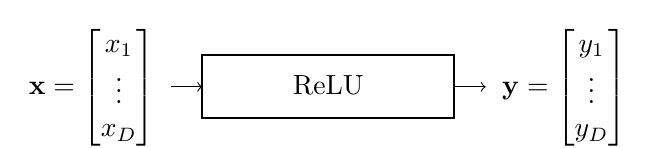
\begin{tikzpicture}
    \pgftext[base, x=   0cm, y= 0cm] {ReLU}; 
    \pgftext[base, x=  -3cm, y= 0cm] {$\mathbf{x} = \begin{bmatrix}x_1\\ \vdots \\x_D\end{bmatrix}$}; 
    \pgftext[base, x=   3cm, y= 0cm] {$\mathbf{y} = \begin{bmatrix}y_1\\ \vdots \\y_D\end{bmatrix}$}; 
    %\pgftext[base, x=   0cm, y=-1cm] {$\mathbf{w}$}; 
    \draw[black,thick] (-1.6cm,-0.3cm) rectangle (1.6cm,0.5cm); 
    \draw[->] ( -2cm, 0.1cm) -- (-1.6cm, 0.1cm);
    \draw[->] (1.6cm, 0.1cm) -- (   2cm, 0.1cm);
    %\draw[->] (  0cm,-0.6cm) -- (   0cm,-0.3cm);
  \end{tikzpicture}
  \end{center}

\noindent
Forward:
\begin{align}
 y_k = \max(x_k, 0) \nonumber
\end{align}

\noindent
Backward:
\begin{align}
 \frac{dy_{k_2}}{dx_{k_1}} &= \delta_{x_{k_1}>0} \hspace{0.3cm} \text{if} \hspace{0.3cm} k_1=k_2 \nonumber \\
                           &= 0 \hspace{0.3cm} \text{otherwise} \nonumber
\end{align}




\subsubsection{Sigmoid}

\section{Normalization functions}
\begin{itemize}
 \item Contrast normalization (forward / backward)
 \item Batch normalization
\end{itemize}


\section{Classification and loss functions}
\subsection{Prediction functions}



\subsubsection{Softmax}
Softmax prediction if rather suited for problems classifying mutually exclusive classes: it forces one class (the ground-truth label) to have a score 
1, the other labels are forced to have a score of 0. 

  \begin{center}
  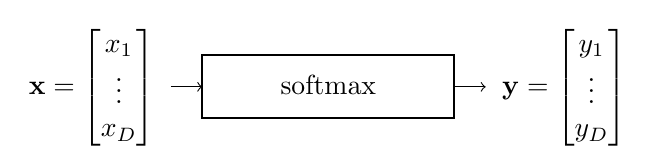
\begin{tikzpicture}
    \pgftext[base, x=   0cm, y= 0cm] {softmax}; 
    \pgftext[base, x=  -3cm, y= 0cm] {$\mathbf{x} = \begin{bmatrix}x_1\\ \vdots \\x_D\end{bmatrix}$}; 
    \pgftext[base, x=   3cm, y= 0cm] {$\mathbf{y} = \begin{bmatrix}y_1\\ \vdots \\y_D\end{bmatrix}$}; 
    %\pgftext[base, x=   0cm, y=-1cm] {$\mathbf{w}$}; 
    \draw[black,thick] (-1.6cm,-0.3cm) rectangle (1.6cm,0.5cm); 
    \draw[->] ( -2cm, 0.1cm) -- (-1.6cm, 0.1cm);
    \draw[->] (1.6cm, 0.1cm) -- (   2cm, 0.1cm);
    %\draw[->] (  0cm,-0.6cm) -- (   0cm,-0.3cm);
  \end{tikzpicture}
  \end{center}

\noindent
\underline{Forward:} 
\begin{align}
 y_k = \frac{e^{x_k}}{\sum_{k'=1}^D e^{x_{k'}}} \nonumber
\end{align}

\noindent
\underline{Backward:}
\begin{align}
 \frac{dy_{k_2}}{dx_{k_1}} = \frac{e^{x_{k_2}}}{\sum_{k=1}^{D}e^{x_k}} \delta_{k_1=k_2} - \frac{e^{x_{k_1}+x_{k_2}}}{(\sum_{k=1}^{D}e^{x_k})^2} 
\nonumber
\end{align}





\subsubsection{Sigmoid}
Sigmoid prediction function is best suited for classification of images with multiple labels: each label gets a score in $[0, 1]$, while the sum is 
not forced to a particular value.

  \begin{center}
  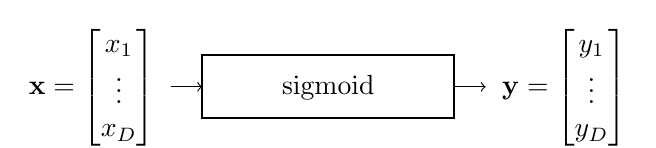
\begin{tikzpicture}
    \pgftext[base, x=   0cm, y= 0cm] {sigmoid}; 
    \pgftext[base, x=  -3cm, y= 0cm] {$\mathbf{x} = \begin{bmatrix}x_1\\ \vdots \\x_D\end{bmatrix}$}; 
    \pgftext[base, x=   3cm, y= 0cm] {$\mathbf{y} = \begin{bmatrix}y_1\\ \vdots \\y_D\end{bmatrix}$}; 
    %\pgftext[base, x=   0cm, y=-1cm] {$\mathbf{w}$}; 
    \draw[black,thick] (-1.6cm,-0.3cm) rectangle (1.6cm,0.5cm); 
    \draw[->] ( -2cm, 0.1cm) -- (-1.6cm, 0.1cm);
    \draw[->] (1.6cm, 0.1cm) -- (   2cm, 0.1cm);
    %\draw[->] (  0cm,-0.6cm) -- (   0cm,-0.3cm);
  \end{tikzpicture}
  \end{center}

\noindent
\underline{Forward:}
\begin{align}
 y_k = \frac{1}{1+e^{-x_k}} \nonumber
\end{align}

\noindent
\underline{Backward:}
\begin{align}
 \frac{dy_{k_2}}{dx_{k_1}} = \frac{e^{-x_{k_2}}}{(1+e^{-x_{k_2}})^2} \delta_{k_1=k_2} \nonumber
\end{align}






%==============================================================================================================
\subsection{Loss functions}


\subsubsection{Classification losses}

\paragraph{\textit{Log-loss}}
Log-loss is generally used with a softmax prediction function. Only the predicted score of the \textit{ground-truth} class is taken into acount. 

  \begin{center}
  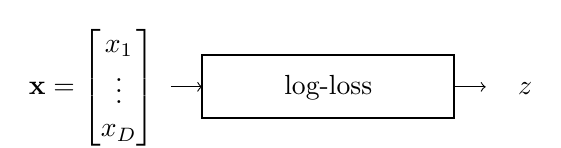
\begin{tikzpicture}
    \pgftext[base, x=   0cm, y= 0cm] {log-loss}; 
    \pgftext[base, x=  -3cm, y= 0cm] {$\mathbf{x} = \begin{bmatrix}x_1\\ \vdots \\x_D\end{bmatrix}$}; 
    \pgftext[base, x= 2.5cm, y= 0cm] {$z$}; 
    %\pgftext[base, x=   0cm, y=-1cm] {$\mathbf{w}$}; 
    \draw[black,thick] (-1.6cm,-0.3cm) rectangle (1.6cm,0.5cm); 
    \draw[->] ( -2cm, 0.1cm) -- (-1.6cm, 0.1cm);
    \draw[->] (1.6cm, 0.1cm) -- (   2cm, 0.1cm);
    %\draw[->] (  0cm,-0.6cm) -- (   0cm,-0.3cm);
  \end{tikzpicture}
  \end{center}

\noindent
\underline{Forward:} 
\begin{align}
 z = - \ln(x_c) \nonumber
\end{align}

\noindent
\underline{Backward:}
\begin{align}
 \frac{dz}{dx_k} = -\frac{1}{x_c} \delta_{k=c} \nonumber
\end{align}


\paragraph{\textit{Cross-entropy}}
Log-loss is generally used with a sigmoid prediction function.  

  \begin{center}
  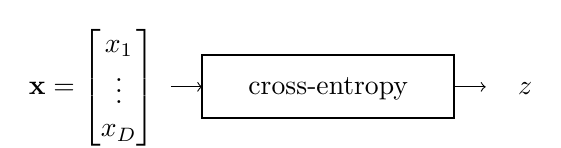
\begin{tikzpicture}
    \pgftext[base, x=   0cm, y= 0cm] {cross-entropy}; 
    \pgftext[base, x=  -3cm, y= 0cm] {$\mathbf{x} = \begin{bmatrix}x_1\\ \vdots \\x_D\end{bmatrix}$}; 
    \pgftext[base, x= 2.5cm, y= 0cm] {$z$}; 
    %\pgftext[base, x=   0cm, y=-1cm] {$\mathbf{w}$}; 
    \draw[black,thick] (-1.6cm,-0.3cm) rectangle (1.6cm,0.5cm); 
    \draw[->] ( -2cm, 0.1cm) -- (-1.6cm, 0.1cm);
    \draw[->] (1.6cm, 0.1cm) -- (   2cm, 0.1cm);
    %\draw[->] (  0cm,-0.6cm) -- (   0cm,-0.3cm);
  \end{tikzpicture}
  \end{center}

\noindent
\underline{Forward:} 
\begin{align}
 z = - \sum_{k=1}^{D} l_k \ln(x_k) \nonumber
\end{align}
where $l_k$ is the ground-truth label of class $k$ for the input image. Here, it should be noticed that for a multiclass problem, the ground-truth labels must be adapted to the cross-entropy formulation. For instance, $l_k = 1$ if class $k$ is present in the input image, $-1$ otherwise. 

\vspace{0.3cm}

\noindent
\underline{Backward:}
\begin{align}
 \frac{dz}{dx_k} = -l_k \frac{1}{x_k} \nonumber
\end{align}




\subsubsection{Regression losses}

\paragraph{\textit{Laptev-style}}
In \cite{Oquab15}, the authors propose a deep structure which is designed to:
\begin{itemize}
 \item localize the objects in the input image;
 \item treat input images of variable sizes.  
\end{itemize}
To achieve these goals, they propose to replace the last fully-connected layers by convolutional blocks. By doing so, there is no need to enforce a fixed input image size: when a larger image than expected is fed to the network, instead of having one vector of $D$ scores for the whole image, the net provides a matrix of $n \times m$ vectors of $D$ scores, where $n \times m$ is the dimension of the output map of the last convolutional layers. In other words, the network can more or less be seen as a classifier used in a sliding window fashion.  

However, the aim remains deciding a \textit{global} label for the whole image, while the previous modification only provides $n \times m$ score vectors. To make a decision over the whole image, a pooling layer is introduced after the last convolutional layers: the pooled score vector (average or max vector over the $n \times m$ spatial locations) is the global image score vector. 
For more details, please refer to the article \cite{Oquab15}. 

In order to train this modified network structure, they also provide an adapted loss formulation, which is as follows: 

  \begin{center}
  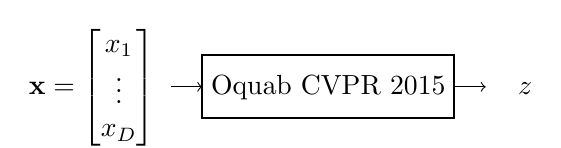
\begin{tikzpicture}
    \pgftext[base, x=   0cm, y= 0cm] {Oquab CVPR 2015}; 
    \pgftext[base, x=  -3cm, y= 0cm] {$\mathbf{x} = \begin{bmatrix}x_1\\ \vdots \\x_D\end{bmatrix}$}; 
    \pgftext[base, x= 2.5cm, y= 0cm] {$z$}; 
    %\pgftext[base, x=   0cm, y=-1cm] {$\mathbf{w}$}; 
    \draw[black,thick] (-1.6cm,-0.3cm) rectangle (1.6cm,0.5cm); 
    \draw[->] ( -2cm, 0.1cm) -- (-1.6cm, 0.1cm);
    \draw[->] (1.6cm, 0.1cm) -- (   2cm, 0.1cm);
    %\draw[->] (  0cm,-0.6cm) -- (   0cm,-0.3cm);
  \end{tikzpicture}
  \end{center}

\noindent
\underline{Forward:}
\begin{align}
 z = \sum_{k=1}^D \ln (1+e^{-l_k x_k}) \nonumber
\end{align}
where $l_k$ is the true label for the presence of object $k$ in the image:
\begin{align}
 \forall k = 1..D, \hspace{0.3cm} 
    l_k &=+1 \hspace{0.3cm} \text{if object $k$ is present in the input image} \nonumber \\
        &=-1 \hspace{0.3cm} \text{if object $k$ is absent from the input image} \nonumber
\end{align}


\noindent
\underline{Backward:}
\begin{align}
 \frac{dz}{dx_k} = \frac{l_k e^{-l_k x_k}}{1+e^{-l_k x_k}} \nonumber
\end{align}






%==============================================================================================================
\subsection{Computational tricks}

\subsubsection{Softmax log-loss combination}

  \begin{center}
  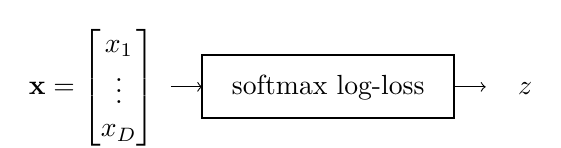
\begin{tikzpicture}
    \pgftext[base, x=   0cm, y= 0cm] {softmax log-loss}; 
    \pgftext[base, x=  -3cm, y= 0cm] {$\mathbf{x} = \begin{bmatrix}x_1\\ \vdots \\x_D\end{bmatrix}$}; 
    \pgftext[base, x= 2.5cm, y= 0cm] {$z$}; 
    %\pgftext[base, x=   0cm, y=-1cm] {$\mathbf{w}$}; 
    \draw[black,thick] (-1.6cm,-0.3cm) rectangle (1.6cm,0.5cm); 
    \draw[->] ( -2cm, 0.1cm) -- (-1.6cm, 0.1cm);
    \draw[->] (1.6cm, 0.1cm) -- (   2cm, 0.1cm);
    %\draw[->] (  0cm,-0.6cm) -- (   0cm,-0.3cm);
  \end{tikzpicture}
  \end{center}
  %
Since softmax involves computing exponentials, the formulation of the ``softmax + log-loss'' can be simplified in order to lighten computational 
cost. 

\noindent
\underline{Forward:} 
\begin{align}
 z = -x_c + \ln( \sum_{k=1}^D e^{x_k} ) \nonumber
\end{align}

\noindent
\underline{Backward:}
\begin{align}
 \frac{dz}{dx_k} = -\delta_{k=c} + \frac{e^{x_k}}{\sum_{k'=1}^D e^{x_{k'}}} \nonumber
\end{align}




\subsubsection{Avoiding computational errors in exponentials}

For the softmax, we need to compute exponentials of matrices. To avoid computational errors, a normalization trick can be used for 
softmax and softmax + log-loss. This normalization is used in MatConvNet. 
For instance, in softmax + log-loss, 

\noindent
\underline{Forward:} 
\begin{align}
  z = -x_c + x_{max} + \ln(\sum_{k=1}^D e^{x_k-x_{max}}) \nonumber
\end{align}

\noindent
\underline{Backward:}
\begin{align}
  \frac{dz}{dx_k} = -\delta_{k=c} + \frac{e^{x_k-x_{max}}}{\sum_{k'=1}^D e^{x_{k'}-x_{max}}} \nonumber
\end{align}
  






%==============================================================================================================

\subsection{Privileged information integrated into classif and loss function}

\subsubsection{What is privileged information?}


\subsubsection{How is privileged information interpreted?}
``Difficulty level'' of the input of interest.\\
Assumption: if an example is easy to classify considering privileged information, then it has to be easy to classify considering common information.
If it is hard to classify considering privileged information, then forcing common classifier to classify it well is a lost cause. Besides, if it is 
difficult in the privileged space, the input example might be an outlier: if so, it would be misleading to force the common classifier to classify it 
well. 

Difficulty level: corresponds to the classification score in the privileged space. 



\subsubsection{Log-loss+}

Here, $\rho$ is a scalar. It is specific to each input image. It is computed as follows:

\begin{align}
 \rho = \langle w_c, x^* \rangle - \max_{k \neq c} \langle w_k, x^* \rangle \nonumber \\
 \rho = \max(\min(\rho, \tau_{max}), \tau_{min}) \nonumber
\end{align}

The $\rho$ is specific to the input image value, and is then integrated in the loss function as follows: 


  \begin{center}
  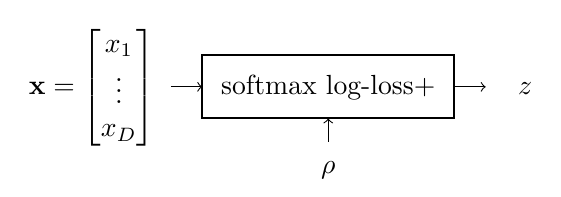
\begin{tikzpicture}
    \pgftext[base, x=   0cm, y= 0cm] {softmax log-loss+}; 
    \pgftext[base, x=  -3cm, y= 0cm] {$\mathbf{x} = \begin{bmatrix}x_1\\ \vdots \\x_D\end{bmatrix}$}; 
    \pgftext[base, x= 2.5cm, y= 0cm] {$z$}; 
    \pgftext[base, x=   0cm, y=-1cm] {$\rho$}; 
    \draw[black,thick] (-1.6cm,-0.3cm) rectangle (1.6cm,0.5cm); 
    \draw[->] ( -2cm, 0.1cm) -- (-1.6cm, 0.1cm);
    \draw[->] (1.6cm, 0.1cm) -- (   2cm, 0.1cm);
    \draw[->] (  0cm,-0.6cm) -- (   0cm,-0.3cm);
  \end{tikzpicture}
  \end{center}

\noindent
\underline{Forward:} 
\begin{align}
 z = -\rho x_c + \rho \ln( \sum_{k=1}^D e^{x_k} ) \nonumber
\end{align}

\noindent
\underline{Backward:}
\begin{align}
 \frac{dz}{dx_k} = -\rho \delta_{k=c} + \rho \frac{e^{x_k}}{\sum_{k'=1}^D e^{x_{k'}}} \nonumber
\end{align}





\subsubsection{Softmax+}

Here, $\rho$ is a vector. It is specific to each input image. It is computed as follows:

\begin{align}
\forall k = 1..D, \hspace{0.2cm}
 &\rho_k = \langle w_k, x^* \rangle \nonumber \\
 &\rho_k = \max(\min(\rho_k, \tau_{max}), \tau_{min}) \nonumber
\end{align}

The $\rho$ is specific to the input image value, and is then integrated in the loss function as follows: 

  \begin{center}
  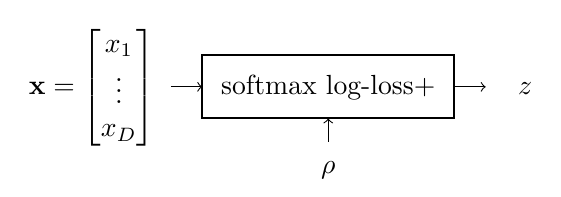
\begin{tikzpicture}
    \pgftext[base, x=   0cm, y= 0cm] {softmax log-loss+}; 
    \pgftext[base, x=  -3cm, y= 0cm] {$\mathbf{x} = \begin{bmatrix}x_1\\ \vdots \\x_D\end{bmatrix}$}; 
    \pgftext[base, x= 2.5cm, y= 0cm] {$z$}; 
    \pgftext[base, x=   0cm, y=-1cm] {$\rho$}; 
    \draw[black,thick] (-1.6cm,-0.3cm) rectangle (1.6cm,0.5cm); 
    \draw[->] ( -2cm, 0.1cm) -- (-1.6cm, 0.1cm);
    \draw[->] (1.6cm, 0.1cm) -- (   2cm, 0.1cm);
    \draw[->] (  0cm,-0.6cm) -- (   0cm,-0.3cm);
  \end{tikzpicture}
  \end{center}

\noindent
\underline{Forward:} 
\begin{align}
 z = -\ln(\rho_c) - x_c + \ln( \sum_{k=1}^D \rho_k e^{x_k} ) \nonumber
\end{align}

\noindent
\underline{Backward:}
\begin{align}
 \frac{dz}{dx_k} = -\delta_{k=c} + \frac{\rho_k e^{x_k}}{\sum_{k'=1}^D \rho_{k'} e^{x_{k'}}} \nonumber
\end{align}





\subsubsection{Loss Inequality Regularization: another approach from the literature}

In \cite{WangCVPR15hiddeninfo}, the authors propose another approach to integrate privileged information into the classification scheme. They propose a framework in which the privileged information is a model for the common information. In other words, the classifier in the common space is forced to be as good as the classifier in the privileged space, however \textit{the classifier in the common space is not allowed to be better than the classifier in the privileged space}. 
This paradigm forces the classifier to be quite efficient, while avoiding overfitting to the outliers. 

For each input image, the loss is computed as follows: 

  \begin{center}
  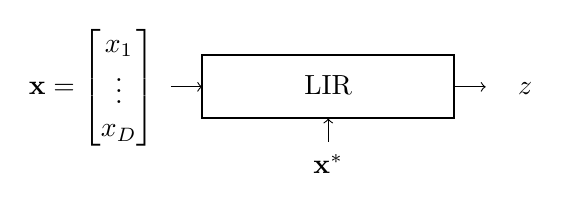
\begin{tikzpicture}
    \pgftext[base, x=   0cm, y= 0cm] {LIR}; 
    \pgftext[base, x=  -3cm, y= 0cm] {$\mathbf{x} = \begin{bmatrix}x_1\\ \vdots \\x_D\end{bmatrix}$}; 
    \pgftext[base, x= 2.5cm, y= 0cm] {$z$}; 
    \pgftext[base, x=   0cm, y=-1cm] {$\mathbf{x^*}$}; 
    \draw[black,thick] (-1.6cm,-0.3cm) rectangle (1.6cm,0.5cm); 
    \draw[->] ( -2cm, 0.1cm) -- (-1.6cm, 0.1cm);
    \draw[->] (1.6cm, 0.1cm) -- (   2cm, 0.1cm);
    \draw[->] (  0cm,-0.6cm) -- (   0cm,-0.3cm);
  \end{tikzpicture}
  \end{center}

\noindent
\underline{Forward:} 
\begin{align}
 z = l(\mathbf{x}) + \eta l(\mathbf{x^*}) + \gamma [ l(\mathbf{x^*}) - l(\mathbf{x}) ]_+ \nonumber 
\end{align}
where $\eta$ and $\gamma$ are two hyper parameters, $[.]_+ = max(0,.)$ and $l$ is a predetermined loss function. 

NB: regularization terms are present in the original formulation of \cite{WangCVPR15hiddeninfo}. In the case of a CNN, no parameter is learned in the classification and loss layers, thus no regularization term is needed. 

\vspace{0.3cm}

\noindent
\underline{Backward:} 

\vspace{0.3cm}

{\color{red}Although this loss formulation is differentiable as soon as the loss $l$ is piecewise differentiable, deriving this function with respect to each $x_k$ would not lead to take into account any privileged information: 
\begin{align}
 \frac{dz}{dx_k} &= (1-\gamma) \frac{dl}{dx_k}(\mathbf{x})  &  \text{if}& \hspace{0.3cm} l(x^*) > l(x) \nonumber \\
                 &= \frac{dl}{dx_k}(\mathbf{x})             &  \text{if}& \hspace{0.3cm} l(x^*) \leq l(x) \nonumber
\end{align}

In the classical formulation, the quantity $\frac{dz}{dx_k} = \frac{dl}{dx_k}(\mathbf{x})$ is backpropagated.
Here, this quantity is backpropagated only when the classifier in the privileged space performs better than the classifier in the common space. 
If the cassifier in the common space is the best, a \textit{lesser} quantity $\frac{dz}{dx_k} = (1-\gamma) \frac{dl}{dx_k}(\mathbf{x})$ is backpropagated.
This observation is totally in contradiction with the philosophy of this approach: since we want to penalize an overfitting classifier (\textit{i.e.} when $l(x) < l(x^*)$), the backpropagated quantity should be higher when $l(x) < l(x^*)$.

Moreover, the backpropagated value only depends on a \textit{condition} over the values $l(x)$ and $l(x^*)$. Since $\gamma$ is a hyper-parameter, the backpropagated value is not adapted to each example: it does not fully exploit the privileged information. 

For both these reasons, this formulation does not seem adapted to a CNN training. 
}

\section{A few training tricks}
\begin{itemize}
 \item dropout
 \item dropconnect
 \item standard values for several hyper parameters:
 \begin{itemize}
  \item weight decay
  \item learning rate(s)
  \item nb epochs
 \end{itemize}

\end{itemize}

\section{Hyper Parameters}

\subsection{Validation}

The objective of learning is not to minimize training error, but to build a model able to generalize well. A good approximation is for sure to minimize the test error, but one should care to not overfit the later. As the process of learning a convnet usually takes three days for medium dataset and sometimes three weeks for the bigest one, people usually create one validation fold instead of five for a normal cross-validation. In fact, the amount of data is so high that it become less important to average the accuracy of 5 fold in order to be sure to not overfit the testing set.

\subsection{Parameters Initilization}

Biases can generally be initialized to zero, but weights need to be initialized carefully to break the symetry between filters of the same convolutional layer. 
... blabla ... However in the case of RBMs?, a zero-mean Gaussian with a small standard deviation around 0.1 or 0.01 works well to initialize the weights.

\subsection{Preprocessing}



\subsection{Learning Rate}

The learning rate is the most important hyperparameter to tune. The optimal learning rate is usually close to (by a factor of 2) the largest learning rate that does not cause divergence of the training criterion. A good heuristic for setting the learning rate is starting with a large learning rate (for instance 5e-1) and if the training criterion diverge, trying again with a 3 times smaller learning rate until no divergence is observed.

Decreasing learning rate

\subsection{Batch size}

With a batch size B equal to 1 the ordinary stochastique (also called online) gradient descent is computed, while with B equal to the training set size this is the standard (also called batch) gradient descent. When B increases we can get more multiply-add operations per second by taking advantage of parallelism or efficient matrix-matrix multiplications. (en revanche) Smaller values of B may benefit from more exploration in parameter space and a form of regularization due to the noise injected in the gradient estimator. Also, stochastic (little mini-batch) gradient descent converges much faster than ordinary (batch) gradient descent. 
Because random access to memory is expensive, a good approximation, is to visit the examples (or mini-batches) in a fixed order corresponding in their order in memory after a unique shuffling step (repeating the examples in the same order for each epoch). Nevertheless, faster convergence has been observed if the training set is shuffled before each epoch.
B = 32 is a goodd default value, with values above 10 taking advantage of the speed-up of matrix-matrix products over matrix-vector products.

\subsection{Epoch number}

early stopping




\section{Optimizer}

SGD :
learning rate
learning rate decay
momentum
momentum nesterov
weight decay L1 L2

L-BFGS
second order

AdaGrad
Duchi, J., Hazan, E., and Singer, Y. (2011). Adap- tive subgradient methods for online learning and stochastic optimization. Journal of Machine Learning Research.


RMSProp (Hinton)

Adadelta (Matthew Zeiler)
Adam?



\section{Reducing overfiting}
Dropout
Dropconnect
Data augmentations

\section{Improving accuracy}
Model ensembles
multi-scale

\section{Improving speed and memory}
size of a batch
batch 3D Tensors versus 4D Tensors
multi GPU

\section{Hyperparameter searching algorithm}
Grid search
Random search (Bengio)

\section{Pretrained models}
Transfer learning
convnet as feature extractor
Fine-Tuning the Convnet
dark Knowledge (Hinton) with model ensembles
    
\section{Other tips}
Sanity checks
monitoring the learning process
how to learn properly without killing neurons
benchmarking
Random seeds
Train on small dataset should be able to overfit to be sure gradient descent is well implemented 




%============================================================
\chapter{Image recognition state of the art CNN architectures}
These networks are state of the art examples of what can be implemented on different datasets. 

In table \ref{table:summary_SoA_nets}, we present an overview of each standard network, then we present all described nets in more details. 


\begin{table}[h]
\begin{center}
 \begin{tabular}{|l|l||c||c|c|c|}
  \hline
  &                                          &                           & \multicolumn{3}{c|}{Number of weights}        \\
  \cline{4-6}
  & Net                                      & Input image size          & Convolutions & Fully-connected & Total       \\
  \hline
  \multirow{3}{*}{Small}
  & LeNet \cite{MNIST}                       & $28 \times 28 \times 1$   & 25,500       & 405,000         & 430,500     \\ 
  & CIFAR-10 \cite{CIFAR}                    & $32 \times 32 \times 3$   & 79,200       & 66,176          & 145,376     \\
  & LR-CNN \cite{Chevalier15}                & $32 \times 32 \times 3$   &  &  & \\
  \hline
  \multirow{3}{*}{Medium}
  & AlexNet \cite{Krizhevsky12}              & $227 \times 227 \times 3$ & 2,332,704    & 58,621,952      & 60,954,656 \\
  & Overfeat large \cite{Sermanet14overfeat} & $221 \times 221 \times 3$ &  &  & \\
  & CNN-M \cite{Chatfield14}                 & $224 \times 224 \times 3$ & 6,526,752 & 96,370,688 & 102,897,440 \\
  \hline
  \multirow{2}{*}{Large}
  & Very deep                                &                           &  &  & \\ 
  & GoogLeNet                                &                           &  &  & \\
  \hline
 \end{tabular}
 \caption{State of the art CNN architectures - summary.}
 \label{table:summary_SoA_nets}
\end{center}
\end{table}









\section{Small networks}

\subsection{LeNet (on MNIST)}

LeNet architecture \cite{MNIST}, described in table \ref{table:LeNet} was initially designed for MNIST image classification, and contains a total of 
\textbf{430,500} learnable weights (25,500 in the convolutional part, 405,000 in the fully-connected part). 

MNIST contains 70,000 images of handwritten digits. These images belong to 10 classes (``0'', ``1'' ... ``9'') and have a size $28 \times 
28 \times 1$ (greyscale images). 

\begin{table}[h]
\begin{center}
 \begin{tabular}{|l||l||l|c|c||l|}
   \hline
   Layer name  & Input                          & Details                                 & Stride & Padding & Output                 \\
   \hline
   \hline
   conv1       & $28 \times 28 \times 1$ images & 20 filters $5 \times 5 \times 1$        & 1      & 0       & 20 maps $24 \times 24$ \\
   pool1       & 20 maps $24 \times 24$         & max on $[2, 2]$ regions                 & 2      & 0       & 20 maps $12 \times 12$ \\
   \hline
   conv2       & 20 maps $12 \times 12$         & 50 filters $5 \times 5 \times 20$       & 1      & 0       & 50 maps $8 \times 8$   \\
   pool2       & 50 maps $8 \times 8$           & max on $[2, 2]$ regions                 & 2      & 0       & 50 maps $4 \times 4$   \\
   \hline
   fc3         & 50 maps $4 \times 4$           & 500 neurons                             &        &         & vector of size 500     \\
   relu3       & vector of size 500             &                                         &        &         & vector of size 500     \\
   fc4         & vector of size 500             & 10 neurons                              &        &         & vector of size 10      \\
   \hline
   sotfmax     & vector of size 10              &                                         &        &         & vector of size 10      \\
   log-loss    & vector of size 10              & only for training                       &        &         & loss value             \\
   \hline
 \end{tabular}
 \caption{Architecture example on MNIST (architecture: LeNet \cite{MNIST}). Total weights: 430,500.}
 \label{table:LeNet}
\end{center}
\end{table} 




\subsection{Standard architecture on CIFAR}

The architecture described in table \ref{table:CIFAR} is a standard architecture used on CIFAR-10 image classification, and contains a total of 
\textbf{145,376} learnable weights (79,200 in the convolutional part, 66,176 in the fully-connected part). 

CIFAR \cite{CIFAR} contains  images centered on objects. These images belong to 10 classes (CIFAR-10) or 100 classes (CIFAR-100) and have a size $32 
\times 32 \times 3$. 

\begin{table}[h]
\begin{center}
 \begin{tabular}{|l||l||l|c|c||l|}
   \hline
   Layer name & Input                          & Details                                 & Stride & Padding   & Output                 \\
   \hline
   \hline
   conv1      & $32 \times 32 \times 3$ images & 32 filters $5 \times 5 \times 3$        & 1      & [2,2;2,2] & 32 maps $32 \times 32$ \\
   pool1      & 32 maps $32 \times 32$         & max on $[3, 3]$ regions                 & 2      & [0,1;0,1] & 32 maps $16 \times 16$ \\
   relu1      & 32 maps $16 \times 16$         &                                         &        &           & 32 maps $16 \times 16$ \\
   \hline
   conv2      & 32 maps $16 \times 16$         & 32 filters $5 \times 5 \times 32$       & 1      & [2,2;2,2] & 32 maps $16 \times 16$ \\
   relu2      & 32 maps $16 \times 16$         &                                         &        &           & 32 maps $16 \times 16$ \\
   pool2      & 32 maps $16 \times 16$         & average on $[3, 3]$ regions             & 2      & [0,1;0,1] & 32 maps $8 \times 8$   \\
   \hline
   conv3      & 32 maps $8 \times 8$           & 64 filters $5 \times 5 \times 32$       & 1      & [2,2;2,2] & 64 maps $8 \times 8$   \\
   relu3      & 64 maps $8 \times 8$           &                                         &        &           & 64 maps $8 \times 8$   \\
   pool3      & 64 maps $8 \times 8$           & average on $[3, 3]$ regions             & 2      & [0,1;0,1] & 64 maps $4 \times 4$   \\
   \hline
   fc4        & 64 maps $4 \times 4$           & 64 neurons                              &        &           & vector of size 64      \\
   fc5        & vector of size 64              & 10 neurons                              &        &           & vector of size 10      \\
   \hline
   sotfmax     & vector of size 10              &                                         &        &         & vector of size 10      \\
   log-loss    & vector of size 10              & only for training                       &        &         & loss value             \\
   \hline
 \end{tabular}
 \caption{Architecture example on CIFAR-10 \cite{CIFAR}. Total weights: 145,376.}
 \label{table:CIFAR}
\end{center}
\end{table} 







\subsection{LR-CNN}

This architecture was proposed in \cite{Chevalier15}. Adapted from the historic AlexNet-like networks, this architecture is designed to recognize 
low resolution images in a fine-grained context. More precisely, this structure has been tested on FGVC-Aircraft images \cite{maji13fine-grained} 
resized to a $32 \times 32 \times 3$ input size. 
This dataset contains 10,000 images belonging to 100 aircraft classes. 

The proposed architecture contains a total of  weights ( in the convolutional part, in the fully-connected part).


\begin{table}[h]
\begin{center}
 \begin{tabular}{|l||l||l|c|c||l|}
   \hline
   Layer name & Input                          & Details                                 & Stride & Padding   & Output                 \\
   \hline
   \hline
   conv1      & $32 \times 32 \times 3$ images & 64 filters $5 \times 5 \times 3$        & 1      & [2,2;2,2] &  \\
   relu1      &                                &                                         &        &           &  \\
   norm1      &                                &                                         &        &           &  \\
   pool1      &                                & max on $[3,3]$ regions                  & 2      & [1,1;1,1] &  \\
   \hline
   conv2      &                                & 64 filters $5 \times 5 \times 64$       & 1      & [2,2;2,2] &  \\
   relu2      &                                &                                         &        &           &  \\
   pool2      &                                & max on $[3,3]$ regions                  & 2      & [1,1;1,1] &  \\
   \hline
   conv3      &                                & 64 filters $3 \times 3 \times 64$       & 1      & 0         &  \\
   relu3      &                                &                                         &        &           &  \\
   pool3      &                                & max on $[3,3]$ regions                  & 2      & [1,1;1,1] &  \\
   \hline
   fc4        & 64 maps of size $3 \times 3$   & 128 neurons                             &        &           & vector of size 128 \\
   relu4      & vector of size 128             &                                         &        &           & vector of size 128 \\
   \hline
   fc5        & vector of size 128             & 100 neurons                             &        &           & vector of size 100 \\
   softmax    & vector of size 100             &                                         &        &           & vector of size 100 \\
   log-loss   & vector of size 100             & only for training                       &        &           & loss value         \\
 \end{tabular}
 \caption{LR-CNN architecture \cite{Chevalier15}. Total weights: .}
 \label{table:LR-CNN}
\end{center}
\end{table} 







%===========================================================================================================================================


\section{Medium networks}



\subsection{AlexNet (Krizhevsky)}
\label{AlexNet}

With their paper \cite{Krizhevsky12}, Krizhevsky et al. have achieved tremendous performances on the ILSVRC12 image classification challenge. This 
paper has definitely caused a re-orientation of all image recognition works towards Convolutional Neural Networks. 

This networks contains a total of \textbf{60,954,656} learnable weights (2,332,704 in the convolutional part, 58,621,952 in the fully-connected part).

In table \ref{table:AlexNet}, we describe the architecture in detail. 
It should be noted that, because of the limited computational material at the time of the publication, the network had to be learned in two threads. 
More precisely, we can see in table \ref{table:AlexNet} that for layers conv4 and conv5, the depth of the filters is \textit{half} the depth of the 
input maps. Indeed, half of those filters were learned on a first GPU, and the other half were learned on a second GPU. Both threads converge then so 
that the fully-connected layers are learned jointly. For more details, see \cite{Krizhevsky12}. 




\begin{table}[h]
\begin{center}
 \begin{tabular}{|l||l||l|c|c||l|}
   \hline
   Layer name & Input                            & Details                                 & Stride & Padding   & Output                   \\
   \hline
   \hline
   conv1      & $227 \times 227 \times 3$ images & 96 filters $11 \times 11 \times 3$      & 4      & 0         & 96 maps $55 \times 55$   \\
   relu1      & 96 maps $55 \times 55$           &                                         &        &           & 96 maps $55 \times 55$   \\
   pool1      & 96 maps $55 \times 55$           & max on $[3,3]$ regions                  & 2      & 0         & 96 maps $27 \times 27$   \\
   norm1      & 96 maps $27 \times 27$           & contrast normalization                  &        &           & 96 maps $27 \times 27$   \\
   \hline
   conv2      & 96 maps $27 \times 27$           & 256 filters $5 \times 5 \times 48$      & 1      & [2,2;2,2] & 256 maps $27 \times 27$  \\
   relu2      & 256 maps $27 \times 27$          &                                         &        &           & 256 maps $27 \times 27$  \\
   pool2      & 256 maps $27 \times 27$          & max on $[3,3]$ regions                  & 2      & 0         & 256 maps $13 \times 13$  \\
   norm2      & 256 maps $13 \times 13$          & contrast normalization                  &        &           & 256 maps $13 \times 13$  \\
   \hline
   conv3      & 256 maps $13 \times 13$          & 384 filters $3 \times 3 \times 256$     & 1      & [1,1;1,1] & 384 maps $13 \times 13$  \\
   relu3      & 384 maps $13 \times 13$          &                                         &        &           & 384 maps $13 \times 13$  \\
   \hline
   conv4      & 384 maps $13 \times 13$          & 384 filters $3 \times 3 \times 192$     & 1      & [1,1;1,1] & 384 maps $13 \times 13$  \\
   relu4      & 384 maps $13 \times 13$          &                                         &        &           & 384 maps $13 \times 13$  \\
   \hline
   conv5      & 384 maps $13 \times 13$          & 256 filters $3 \times 3 \times 192$     & 1      & [1,1;1,1] & 256 maps $13 \times 13$  \\
   relu5      & 256 maps $13 \times 13$          &                                         &        &           & 256 maps $13 \times 13$  \\
   pool5      & 256 maps $13 \times 13$          & max on $[3,3]$ regions                  & 2      & 0         & 256 maps $6 \times 6$    \\
   \hline
   fc6        & 512 maps $6 \times 6$            & 4,096 neurons                           &        &           & vector of size 4,096     \\
   relu6      & vector of size 4,096             &                                         &        &           & vector of size 4,096     \\
   \hline
   fc7        & vector of size 4,096             & 4,096 neurons                           &        &           & vector of size 4,096     \\
   relu7      & vector of size 4,096             &                                         &        &           & vector of size 4,096     \\
   \hline
   fc8        & vector of size 4,096             & 1,000 neurons                           &        &           & vector of size 1,000     \\
   softmax    & vector of size 1,000             &                                         &        &           & vector of size 1,000     \\
   log-loss   & vector of size 1,000             & only for training                       &        &           & loss value               \\
   \hline 
 \end{tabular}
 \caption{AlexNet architecture \cite{Krizhevsky12}. Total weights: 60,954,656.}
 \label{table:AlexNet}
\end{center}
\end{table} 







\subsection{Overfeat}

Overfeat is a deep architecture proposed in \cite{Sermanet14overfeat} to classify images from various standard datasets (PASCALVOC, ImageNet...). The 
structure is described in table \ref{table:Overfeat}. The net contains a total of \textbf{} learnable weights ( in the convolutional part,  in 
the fully-connected part).

Overfeat can easily be used as a feature extractor, since the pretrained weights are available online\footnote{Overfeat webpage: 
\url{http://cilvr.nyu.edu/doku.php?id=software:overfeat:start}}. 
Two variants of architectures have been proposed: a fast version (quite fast to compute but not the most accurate) and a large version (the most 
accurate but the slowest version). Here, we detail the large version. 

\begin{table}[h]
\begin{center}
 \begin{tabular}{|l||l||l|c|c||l|}
   \hline
   Layer name & Input                            & Details                                 & Stride & Padding   & Output                   \\
   \hline
   \hline
   conv1      & $221 \times 221 \times 3$ images & 96 filters $7 \times 7$                 & 2      &           & 96 maps                  \\
   relu1      &                                  &                                         &        &           &                          \\
   pool1      &                                  & max on $[3,3]$ regions                  & 3      & 0         & 96 maps $36 \times 36$   \\
   \hline
   conv2      & 96 maps $36 \times 36$           & 256 filters $7 \times 7$                & 1      &           & 256 maps                 \\
   relu2      &                                  &                                         &        &           &                          \\
   pool2      &                                  & max on $[2,2]$ regions                  & 2      & 0         & 256 maps $15 \times 15$  \\
   \hline
   conv3      & 256 maps $15 \times 15$          & 512 filters $3 \times 3$                & 1      & [1,1;1,1] &                          \\
   relu3      &                                  &                                         &        &           & 512 maps $15 \times 15$  \\
   \hline
   conv4      & 512 maps $15 \times 15$          & 512 filters $3 \times 3$                & 1      & [1,1;1,1] &                          \\
   relu4      &                                  &                                         &        &           & 512 maps $15 \times 15$  \\
   \hline
   conv5      & 512 maps $15 \times 15$          & 1,024 filters $3 \times 3$              & 1      & [1,1;1,1] &                          \\
   relu5      &                                  &                                         &        &           & 1,024 maps $15 \times 15$\\
   \hline
   conv6      & 1,024 maps $15 \times 15$        & 1,024 filters $3 \times 3$              & 1      & [1,1;1,1] &                          \\
   relu6      &                                  &                                         &        &           &                          \\
   pool6      &                                  & max on $[3,3]$ regions                  & 3      & 0         & 1,024 maps $5 \times 5$  \\
   \hline     
   fc7        & 1,024 maps $5 \times 5$          & 4,096 filters $5 \times 5$              & 1      &           & vector of size 4,096     \\
   relu7      &                                  &                                         &        &           & vector of size 4,096     \\
   \hline
   fc8        & vector of size 4,096             & 4,096 neurons                           &        &           & vector of size 4,096     \\ 
   relu8      & vector of size 4,096             &                                         &        &           & vector of size 4,096     \\
   \hline
   fc9        & vector of size 4,096             & 1,000 neurons                           &        &           & vector of size 1,000     \\
   softmax    & vector of size 1,000             &                                         &        &           & vector of size 1,000     \\
   ????       & vector of size 1,000             &                                         &        &           & loss value               \\
   \hline
 \end{tabular}
 \caption{Overfeat (large) architecture \cite{Sermanet14overfeat}. Total weights: .}
 \label{table:Overfeat}
\end{center}
\end{table} 





\subsection{CNN-M (Chatfield)}

In their paper \cite{Chatfield14}, Chatfield et al. propose a study comparing Fisher Vectors representations to deep representations on 
PASCALVOC2007. In this context, they present three architectures: CNN-F (fast but not the most accurate), CNN-M (medium, quite accurate), CNN-S 
(slow but not much more accurate than CNN-M). In this report, we describe the CNN-M architecture (which is used throughout \cite{Chatfield14} as 
the reference method). 

This network contains \textbf{102,897,440} learnable weights (6,526,752 in the convolutional part, 96,370,688 in the fully-connected part). It is 
worth noticing that the authors propose ``lighter'' versions of their network by reducing the size of fc7: CNN-M-2048 has 2048 neurons in fc7 (total 
weights: 92,460,832), CNN-M-1024 has 1024 neurons in fc7 (total weights: 87,242,528), CNN-M-128 has 128 neurons in fc7 (total weights: 82,676,512). 
CNN-M has however been widely used for comparative studies in other works \cite{}. 

This architecture was designed to classify ImageNet ILSVRC12 images \cite{Deng09ImageNet}: these 1,2 million images belong to 1,000 classes. 
The weights of this network have been learned on ILSVRC12 data and are online available\footnote{CNN-M pretrained weigths: 
\url{http://www.vlfeat.org/matconvnet/pretrained/}}.

It should be noted that CNN-M is quite similar to AlexNet (described in section \ref{AlexNet}). However, CNN-M is much larger (larger filter banks in 
conv3, conv4, conv5) and reduces much less available information in the first layers (in conv1, stride 2 for CNN-M vs. stride 4 in AlexNet).


\begin{table}[h]
\begin{center}
 \begin{tabular}{|l||l||l|c|c||l|}
   \hline
   Layer name & Input                            & Details                                 & Stride & Padding   & Output                   \\
   \hline
   \hline
   conv1      & $224 \times 224 \times 3$ images & 96 filters $7 \times 7 \times 3$        & 2      & 0         & 96 maps $109 \times 109$ \\
   relu1      & 96 maps $109 \times 109$         &                                         &        &           & 96 maps $109 \times 109$ \\
   norm1      & 96 maps $109 \times 109$         & contrast normalization                  &        &           & 96 maps $109 \times 109$ \\
   pool1      & 96 maps $109 \times 109$         & max on $[3,3]$ regions                  & 2      & 0         & 96 maps $54 \times 54$   \\
   \hline
   conv2      & 96 maps $54 \times 54$           & 256 filters $5 \times 5 \times 96$      & 2      & [1,1;1,1] & 256 maps $26 \times 26$  \\
   relu2      & 256 maps $26 \times 26$          &                                         &        &           & 256 maps $26 \times 26$  \\
   norm2      & 256 maps $26 \times 26$          & contrast normalization                  &        &           & 256 maps $26 \times 26$  \\
   pool2      & 256 maps $26 \times 26$          & max on $[3,3]$ regions                  & 2      & [0,1;0,1] & 256 maps $13 \times 13$  \\
   \hline
   conv3      & 256 maps $13 \times 13$          & 512 filters $3 \times 3 \times 256$     & 1      & [1,1;1,1] & 512 maps $13 \times 13$  \\
   relu3      & 512 maps $13 \times 13$          &                                         &        &           & 512 maps $13 \times 13$  \\
   \hline
   conv4      & 512 maps $13 \times 13$          & 512 filters $3 \times 3 \times 256$     & 1      & [1,1;1,1] & 512 maps $13 \times 13$  \\
   relu4      & 512 maps $13 \times 13$          &                                         &        &           & 512 maps $13 \times 13$  \\
   \hline
   conv5      & 512 maps $13 \times 13$          & 512 filters $3 \times 3 \times 256$     & 1      & [1,1;1,1] & 512 maps $13 \times 13$  \\
   relu5      & 512 maps $13 \times 13$          &                                         &        &           & 512 maps $13 \times 13$  \\
   pool5      & 512 maps $13 \times 13$          & max on $[3,3]$ regions                  & 2      & 0         & 512 maps $6 \times 6$    \\
   \hline
   fc6        & 512 maps $6 \times 6$            & 4,096 neurons                           &        &           & vector of size 4,096     \\
   relu6      & vector of size 4,096             &                                         &        &           & vector of size 4,096     \\
   \hline
   fc7        & vector of size 4,096             & 4,096 neurons                           &        &           & vector of size 4,096     \\
   relu7      & vector of size 4,096             &                                         &        &           & vector of size 4,096     \\
   \hline
   fc8        & vector of size 4,096             & 1,000 neurons                           &        &           & vector of size 1,000     \\
   softmax    & vector of size 1,000             &                                         &        &           & vector of size 1,000     \\
   log-loss   & vector of size 1,000             & only for training                       &        &           & loss value               \\
   \hline 
 \end{tabular}
 \caption{CNN-M architecture \cite{Chatfield14}. Total weights: 102,897,440.}
 \label{table:CIFAR}
\end{center}
\end{table} 









%===========================================================================================================================================

\section{Large networks}

\subsection{Very deep (Zisserman)}

\subsection{GoogLeNet}









%===========================================================
\chapter{Deep nets libraries}
\label{lib}

\section{MatConvNet}
\url{http://www.vlfeat.org/matconvnet/}
\cite{arXiv:1412.4564}

\begin{itemize}
 \item CPU / GPU
 \item Computation times
 \item What is coded for GPU? Where is the big computational improvement of GPU implementation? (A priori convolutions = bottleneck). 
 \item How are convolutions implemented (matricial computation)?
 \item MatLab interface / CUDA + C++
 \item Organization: blocks. To each computational block corresponds a MatLab function. 
 \item If a function does not exist, it can easily be defined by the user. Requirements: forward and backward formulations. Then, it is just another 
block in the backpropagation chain. 
 \item dropout implemented as a layer
 \item 
\end{itemize}

\section{Torch}
{\color{red}Michael \& Remi}

\url{http://torch.ch/}

pros :
\begin{itemize}
 \item easy to shift from CPU to GPU
 \item fast scripting language, LuaJIT
 \item C/CUDA implementation
 \item amazing interface to C, via LuaJIT
 \item maximum flexibility in implementing complex neural network topologies (parallelize nets over CPUs and GPUs)
 \item embeddable, with ports to iOS, Android and FPGA backends
\end{itemize}

cons : 
\begin{itemize}
  \item learning lua 
  \item even with luarocks (package managing) still difficult to deal with libraries (for instance math.round doesn't exist, but math.ceil and math.floor do)
  \item torch.optim, which contain adagrad, rmsprop, sgd, etc., is difficult to use and modify
  \item great ml lib doesn't exist, for instance it's still hard to use a simple SVM
\end{itemize}



\section{Caffe}
{\color{red}Thibaut}









% To start a new column (but not a new page) and help balance the last-page
% column length use \vfill\pagebreak.
% -------------------------------------------------------------------------
%\vfill
%\pagebreak
	
% References should be produced using the bibtex program from suitable
% BiBTeX files (here: refs). The IEEEbib.bst bibliography
% style file from IEEE produces unsorted bibliography list.
% -------------------------------------------------------------------------
\bibliographystyle{IEEEbib}
\bibliography{egbib}

\end{document}
